\chapter{CMS Detector}\label{sec:detectors}
Since the discovery of the neutron in the 30s, humanity's aspiration to understand the most fundamental constituents and laws of physics has only accelerated.
The Discovery of pions, Kaons, and other hadrons from the cosmic rays in the 40s and 50s led to an understanding of the substructure of particles, which culminated in Gell-Mann's Eightfold way.
Deep inelastic scattering performed in the 60s by the Stanford Linear Accelerator Center (SLAC) confirmed the existence of ``partons'' or ``quarks'' of those particles.
Observance of \PJGy and $\Upsilon$ mesons in SLAC and MIT put the third-generation fermions in the collection of particles.
Gargamelle bubble chamber in CERN succeeded in detecting muon neutrinos, postulated by Pauli in the 30s from the beta decay experiment.
CERN's UA1 and UA2 in the 80s confirmed the existence of the first particles in the electroweak scale, namely the W and Z bosonsFermilab's CDF and D0 in the 90s confirmed the existence of the top quark, the heaviest particle in the SM.
Fermilab's CDF and D0 in the 90s confirmed the existence of \PQt , the heaviest particle in the SM.
As much as we appreciate the predecessor physicists for their phenomenal analytic and statistical works, we also need to appreciate the experimental apparatus's evolution.
Although the simple design of a bubble chamber or detection of cosmic rays is still a helpful insight for particle physics research, physicists wanted to create the cosmic and very early phase of the universe on our terra.
Progress from the linear accelerator to the TeV scale circular high energy accelerator was achieved by physicists, engineers, and others.
Its pinnacle came with the construction of the LHC, situated in CERN, the home of UA(1-5).


\section{The LHC and CMS}
The LHC is the world's largest and highest-energy particle collider.
The LHC was built for a decade, from 1998 to 2008.
The construction was completed in collaboration with 100 countries and 10000 scientists around the globe, demonstrating the ethos of global cooperation of the physics community and its majestic scale.
The LHC construction, which costed 5 billion US Dollars for its construction, costs 5.5 billion dollars per year for its electric and computing power consumption \cite{LHCweb}.
The LHC is built in a tunnel 328 feet underground at CERN, on the Franco-Swiss border near Annecy, France, and  Geneva, Switzerland.
The LHC shoots bunches of protons and lead(Pb) ions near the speed of light, enabled by the 27 km ring of superconducting magnets with several accelerating apparatuses.
One can infer the LHC name's origin, given that it is 27km long, shoots hadrons of protons, and collides with each other at 0.9997 fractions of the speed of light.

CERN is an accelerator complex that includes a succession of increasingly higher-energy machines.
\begin{figure}[h!]
	\caption{Picture of the CERN complex \cite{CERN}}
  \label{fig:CERN}
  \centering
  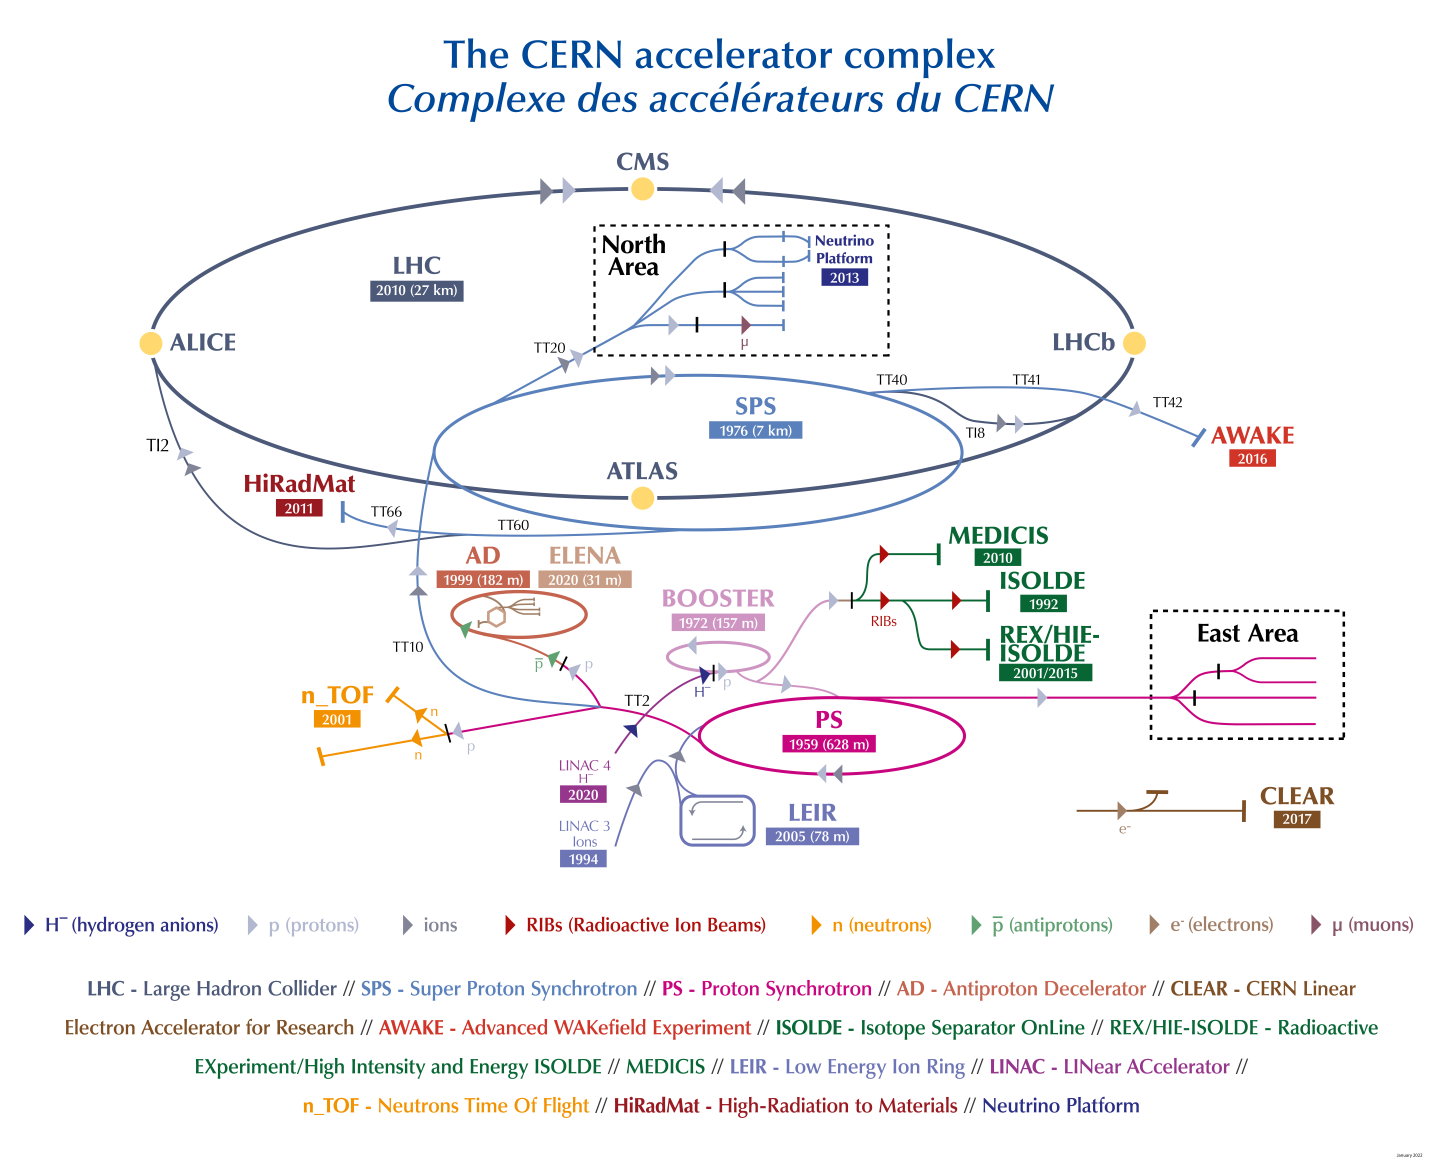
\includegraphics[width=1.0\linewidth]{figs/LHC.png}
\end{figure}
Each machine accelerates a beam of particles to a threshold of desired energy and injects the beam into the next machine in the chain.
The next machine brings the beam to even higher energy and repeats the cycle until it enters the LHC.
The LHC is the last element of this chain, in which the beams reach their highest energies.
The LHC is cooled to 1.9K and maintained at ultrahigh vacuum status.

The goal of LHC was to discover the last remaining piece of the SM, the Higgs boson.
The LHC accomplished its primary goal with the discovery of the Higgs boson by CMS and ATLAS on July 4th, 2012.
However, the LHC's goal does not stop there.
As mentioned in chapter \ref{sec:theory}, several unanswered questions in high energy physics still exist.
LHC wants to address them. It wants to discover the SUSY particles, dark matter, and other exotic particles to help us better understand the most fundamental nature of the universe.

In order to tackle these issues more efficiently, there are four main detectors in the LHC: Compact Muon Solenoid (CMS), A Toroidal LHC Apparatus (ATLAS), A Large Ion Collider Experiment (ALICE), and LHCb.
CMS and ATLAS are general-purpose colliders. They were used for the discovery of the Higgs Boson in 2012. They are used for an entire range of high energy physics, investigating the SUSY particles to dark matter to precision QCD to Lepton Universality.
ALICE is a lead-lead collider, targeting to study a phase of matter called the Quark-Gluon Plasma (QGP). A study of QGP helps us better understand quarks and gluons' behavior when they escape the confinement of the QCD.
Similar research is done in Brookhaven National Laboratory's Pioneering High Energy Nuclear Interaction eXperiment (BNL's PHENIX).
LHCb is a b-factory. It wants to test or challenge ``Lepton Universality,'' claiming that interaction between leptons and a gauge boson measures the same for each lepton.
Similar research is done in BaBar of SLAC and BelleII of KoEnerugi Kasokuki kenkyu kiko (KEK).

The analysis of this dissertation entirely derives from data obtained in CMS.
The following subsections detail the parts and functions of each part of CMS.
\begin{figure}[h!]
	\caption{Picture of CMS viewed from the beam direction \cite{det}}
  \label{fig:cms}
  \centering
  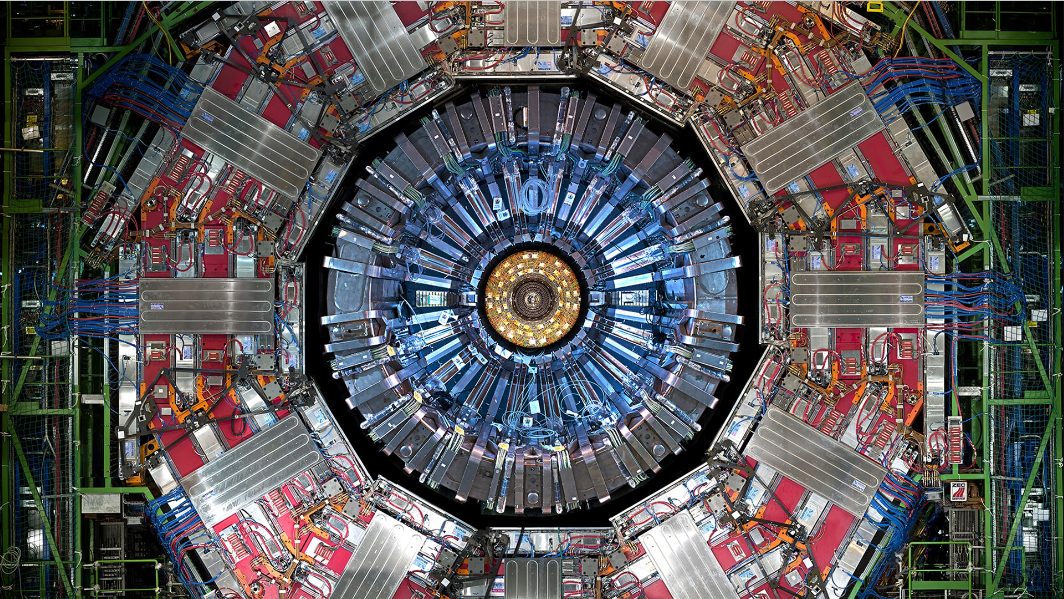
\includegraphics[width=1.0\linewidth]{figs/cms.png}
\end{figure}
CMS consists of 5 main parts: the tracker, the electromagnetic calorimeter (ECAL), the hadronic calorimeter (HCAL), the superconducting magnet, and the Muon chamber.
\begin{figure}[h!]
	\caption{Cartoon of CMS with its subpart annotated \cite{xsec}}
  \label{fig:CMS}
  \centering
  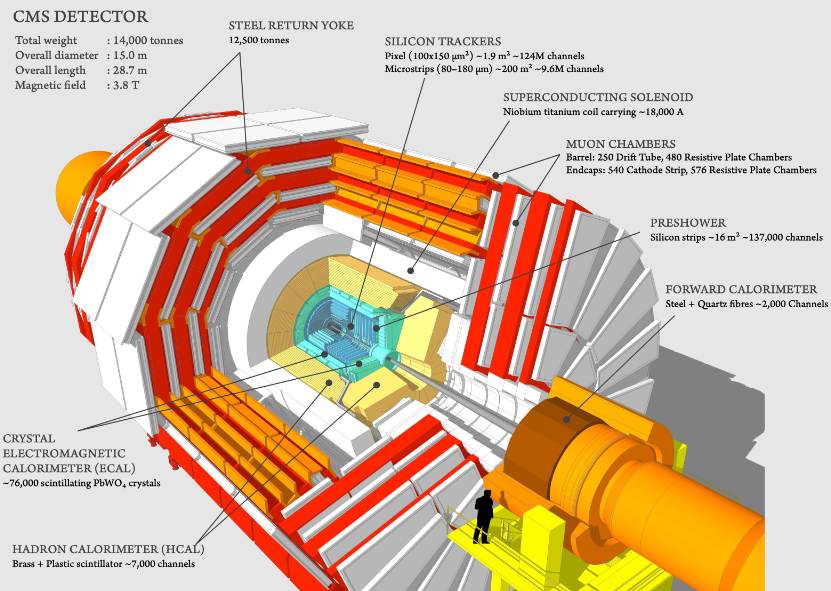
\includegraphics[width=0.87\linewidth]{figs/CMS.png}
\end{figure}
We will review each part's hardware information and its role in the entire CMS.
The review order is identical to a particle's trajectory from the beamspot as in figure \ref{fig:cmsxsec}, except that the tracker is placed at the end for its connection to my analysis' trigger strategy.
\begin{figure}[h!]
  \caption{Cross-section of CMS detector as a particle traverses through the apparatus \cite{xsec}}
  \label{fig:cmsxsec}
  \centering
  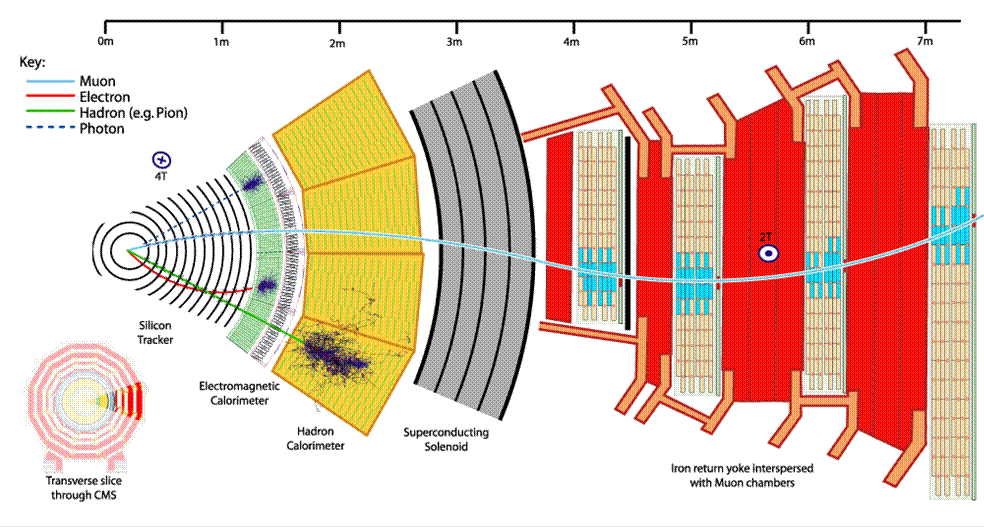
\includegraphics[width=0.87\linewidth]{figs/cmsxsec.png}
\end{figure}
\subsection{Calorimetry}
\subsubsection{ECAL of CMS}
\begin{figure}[h!]
  \caption{Schematic view of the ECAL. \cite{ecal}}
  \label{fig:ECAL}
  \centering
  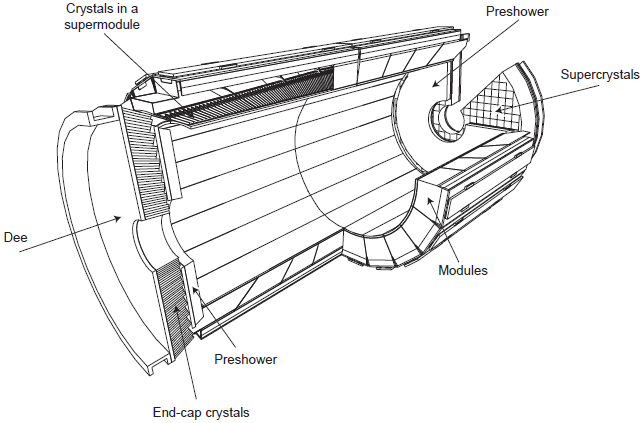
\includegraphics[width=0.87\linewidth]{figs/ECAL.png}
\end{figure}
Electron and photon energies are measured in the ECAL with high precision. 
CMS has a compact scintillating crystal calorimeter with excellent performance for energy resolution. 
The ECAL consists of 75,000 lead-tungstate (PbWO4) crystals with coverage in pseudorapidity up to 3.0. As photons and electrons shower through the crystals, their radiation light is detected by silicon avalanche photodiodes (APDs) in the barrel and vacuum phototriodes (VPTs) in the endcap.
ECAL distinguishes photons from electrons based on the energy dispersion on the i$\eta$-i$\phi$ map as the photon's energy is deposited into a wider area.
ECAL can also distinguish $\pi^{0}$, which decay into two photons, from photons originating from the hard scattering.
ECAL's pre shower system installed in the front of the endcap is used for $\pi^{0}$ rejection and the detection of photons.

\subsubsection{HCAL of CMS}
\begin{figure}[h!]
  \caption{Cross-section of the HCAL in CMS detector. It shows the Barrel, endcap, front, and outside portions. \cite{hcal}}
  \label{fig:HCAL}
  \centering
  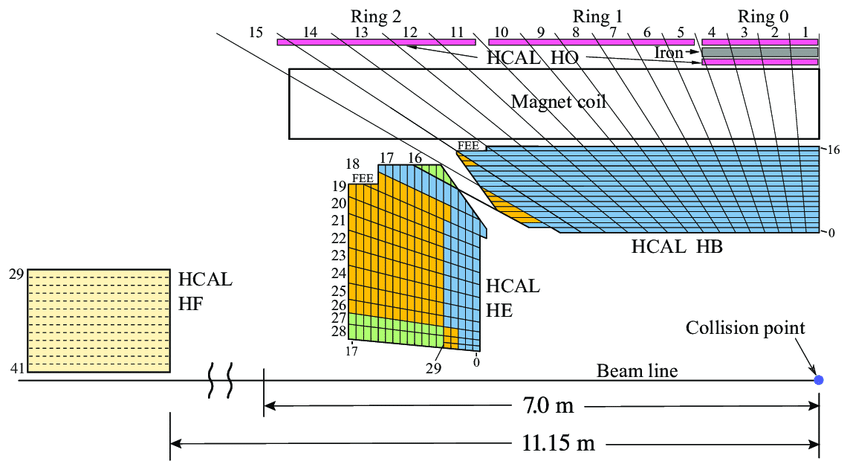
\includegraphics[width=0.87\linewidth]{figs/HCAL.png}
\end{figure}
The ECAL is surrounded by brass/scintillator sampling Hadron Calorimeter (HCAL) with pseudorapidity ($\eta$) up to 3.0.
Strongly interacting SM particles, such as quarks, and gluons, deposit their energy into the HCAL.
Due to the color confinement of QCD, these particles are in the form of hadrons, and hadrons' shower is messier than electromagnetically interacting particles.
We identify these strongly interacting particles as a jet, a narrow cone of hadrons, and other particles produced by the hadronization of a quark or gluon.
HCAL plays an essential role in identifying and measuring neutrinos by measuring jets' energy and direction.
Since the initial momentum in the transverse plane (xy-plane), which is a plane perpendicular ($\perp$) to the beam ($\hat{z}$) direction, is 0, the final transverse momentum is also equal to 0.
Suppose the final transverse momentum is not equal to 0, or there is missing transverse energy (MET), \MET. In that case, it means there is an undetected particle leaving the collider in the opposite direction of all other detected particles' momentum vector summation, signaling the identification of neutrinos.
However, it could also be interpreted as a sign of a BSM particle based on other information.
Thus, \MET plays a crucial role in finding new BSM particles, like the supersymmetric partners of quarks and gluons.
In addition, precise measurement of high energy jets is vital for searches for high mass Standard Model and SMEFT study.

Since HCAL plays such a crucial role in detecting new physics, the structure of HCAL is also highly complex.
Wavelength-shifting (WLS) fibers transport the scintillation light produced by the scintillator tiles to photodetectors.
This light is detected by hybrid photodiodes (HPDs) that can operate in high axial magnetic fields.
While most of the HCAL's Barrel (HB) and endcap (HE) are positioned inside CMS magnet, HCAL outside and front (HO,HF) are located outside the magnet to detect particles from high-energy showers.
The HB and HE sample calorimeters are with 50 mm
thick copper absorber plates interleaved with 4 mm thick scintillator sheets.
The HCAL's Barrel is complemented by a ``tail-catcher'' to ensure that hadronic showers are sampled with nearly 11 hadronic interaction lengths to contain high-energy jets.
HF is installed at each end of CMS detector, which provides coverage up to a pseudorapidity of 5.0, with steel absorber plates used for the harsher radiation environment of the forward systems.
The HF ensures full geometric coverage for measuring the transverse energy in the event.
HCAL's comprehensive geometrical coverage and precise energy measurements are crucial for BSM searches in Vector-Boson Fusion (VBF) Higgs production mode, where high energetic jets decay back-to-back at high pseudorapidity.
Muons and tau leptons deposit only a tiny fraction of their energy in the calorimeters and are identified with tracking and muon detector subsystems' information at the reconstruction level.

\subsection{The superconducting Magnet  of CMS}
The superconducting magnet encompasses the inner tracker and the calorimetry, while outside of the superconducting magnet is the flux return system and muon detector.
The superconducting magnet is 13m-long, 5.9 m inner diameter, 12 kilo-ton, 4 T, the core part of CMS.
CMS magnet system consists of a superconducting coil, the magnet yoke (barrel and endcap), a vacuum tank, ancillaries such as cryogenics, power supplies, and process controls.
The magnetic flux is returned via a 1.5 m thick saturated iron yoke interleaved in four stations of Muon Chamber.

The magnetic field provided by the superconducting magnet is essential for the momentum measurement of charged particles.
Electrically charged particles' trajectories are bent inside the magnetic field due to the Lorentz force.
The particles leave their trajectories in the tracker. 
Furthermore, the trajectory is used to calculate the momentum of each particle.
The 4T magnetic field also enables the detection of isolated electrons produced by the decay of \PQb, W, and Z particles.
CMS ECAL uses these electrons for calibration accuracy to a fraction of a percent.
\subsection{The Muon Chamber of CMS}
\begin{figure}[h!]
	\caption{Cross-section of the Muon Chamer in CMS detector. It shows the 4 layers of the drift tube (DT) cross-section viewed from the z-axis. \cite{det}}
  \label{fig:MC}
  \centering
  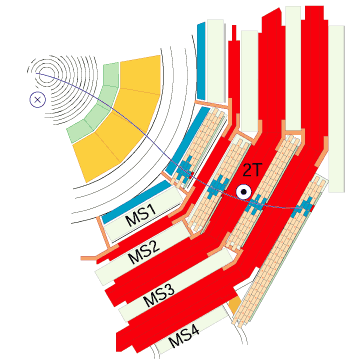
\includegraphics[width=0.4\linewidth]{figs/MCcms.png}
\end{figure}

Muons, stable in CMS perspective due to their lifetime, provide clean signatures, unlike hadrons.
Muon system's reconstruction efficiency is better than 98\% over the full pseudorapidity range.
Each muon station has several layers of aluminum drift tubes (DT) for the barrel region and cathode strip chambers (CSCs) for the endcap region.
The DT and CSC detectors are used to obtain a precise measurement of the four vectors of the muons.
The DT and CSC are complemented by resistive plate chambers (RPCs), fast gaseous muon detectors that provide a muon trigger system.
The considerable thickness of the absorber material (iron) ensures muons do not escape the detector, thereby increasing its identification efficiency.

Muons detected and triggered by the Muon Chamber feed into muon reconstruction algorithms.
In reconstruction algorithms, position, direction vectors, and an estimate of the transverse muon momentum are used as seeds for the track fits using the Kalman filter technique.
The result is a collection of reco::track objects, reconstructed as ``standalone muons.''
For each standalone muon track, a search for tracks matching it among those reconstructed in the inner tracking system (``inner tracks'' or ``silicon tracks'')  is performed.
Based on the Kalman filter technique, the best-matching tracker track and ``standalone muon'' pair gives a collection of reco::Track objects referred to as ``global muons.''
A complementary approach considers all tracker tracks to be potential muon candidates. 
It provides a collection of reco::Track objects referred to as ``tracker muons.''  with compatible signatures in the calorimeters and the muon system.

\section{Tracker of CMS}
\begin{figure}[h!]
	\caption{Cross-section of the trackers in CMS detector. It shows the pixels in the inner tracker for more precise vertexing and the silicon strips on the outer trackers. Silicon strips are tilted with respect to previous layers of strips. \cite{trk}}
  \label{fig:tracker}
  \centering
  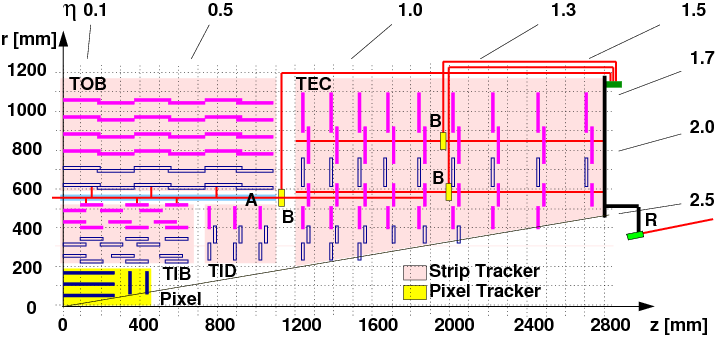
\includegraphics[width=0.9\linewidth]{figs/Tracker.png}
\end{figure}

The inner tracker is the first detector material sitting around the LHC beampipe.
It consists of the pixel cells in the innermost part and silicon strip sensors in the outer part of the tracker.
The innermost tracking material consists of 3 layers of silicon pixel detectors.
In the year of 2017 of Run 2, an additional pixel layer was added for even better performance.
The square pixel detectors with high granularity are extremely radiation resistant and provide the most accurate position information.
The outer layers of the tracker consist of strip sensors, which are more financially affordable.
They are 5.8 m in length, 2.6m in diameter, in ten layers, and consist of 25,000 silicon strip sensors in a cylindrical shape.
The system provides analog data from about 10 million channels.
Each layer is oriented to a slight off-angle to the previous layer for 2D position measurement.

CMS tracking system, with the magnetic field coming from the superconducting magnet, reconstruct muons, electrons, and charged hadrons' tracks with high momentum resolution with an efficiency better than 98\% in pseudorapidity up to 2.5.
They provide the required granularity and precision to deal with high-track multiplicities.
For muons, with information from the measurements of the muon chamber, the tracking system contributes to even better resolution.

The tracker is quintessential for many physics analyses.
Its closest placement to the interaction point provides precise vertex reconstruction and measurement of the tracks' impact parameter (IP).
The trackers' reconstruction for secondary vertices is critical for b-tagging, a method of detecting jets arising from \PQb decays.
It is a frequently used tool in many CMS groups.
For instance, physicists studying Lepton Universality use b-tagging, enabled by the tracker's good vertex reconstruction efficiency, to identify the physics process involving B mesons to Kaons.
In addition, physicists use b-tagging to identify top quarks.
Top quarks predominantly decay into b-jets and are good portals for BSM physics along with the Higgs boson.
The tracker's impact parameter values also play a significant role in discovering BSM physics targetting for LLPs.
LLPs IP values are starkly different from SM particles' IP values.


\section{Trigger of CMS}
\begin{figure}[h!]
	\caption{Cartoon diagram displaying the Trigger and Data Acquisition System process, along with parking of datasets/}
  \label{fig:trig}
  \centering
  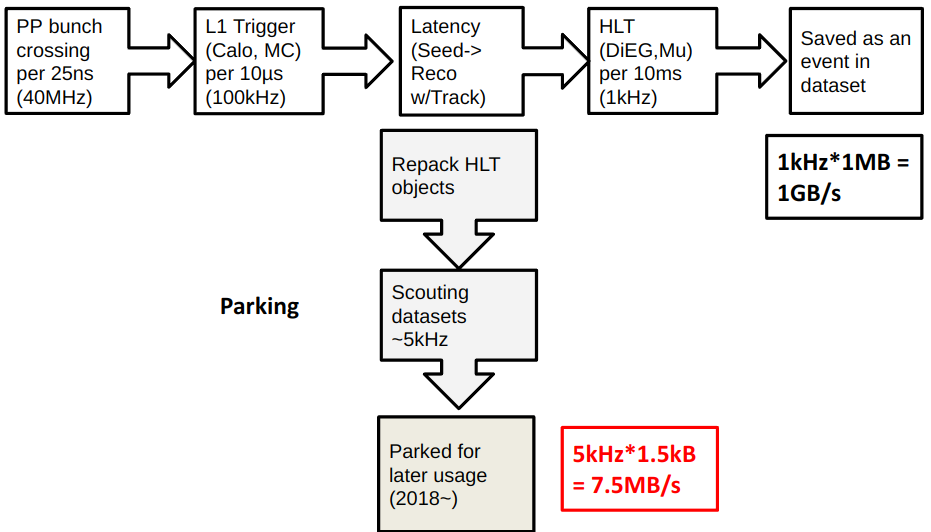
\includegraphics[width=0.95\linewidth]{figs/Trig.png}
\end{figure}
The Discovery of new physics requires high energy and extensive statistics.
New physics, as it has not been discovered so far, has a minimal cross-section.
Extensive statistics are necessary to confirm the existence of the small cross-section signal over standard model backgrounds.
In order to achieve the high statistics, CMS beam crossing happens at a very high rate with bunches of protons shooted together.
CMS beam crossings occur at a rate of 40 million per second (40MHz) with a spacing of 25ns, while 25-50 bunch crossings are usual figures for Run 2 data of CMS.
It totals about 1 billion events occurring in CMS detector per second.

Proton-proton interactions are messy and produce many tracks, given their QCD nature.
However, most of the events are ``not interesting'' to even be considered candidates for potentially interesting events.
These events occur too quickly to be recorded and would take up vast amounts of disk space to store, which would be a waste of electronic resources.
In order to filter and save only ``interesting'' events in the extreme environment, CMS employs the Trigger and Data Acquisition System.
It selects the most interesting hundred or so events per second for storage with fast electronics and resolution.
CMS Data Acquisition System and Triggering are described below.

The first level of triggering, Level 1 (L1), is a hardware trigger.
It uses hardware processors to rapidly select or reject events based on information from the ECAL and Muon Chamber.
The Level 1 trigger reduces the event rate from 40MHz to 100kHz.
An event passing the L1 trigger is transmitted to the Data Acquisition System.
In addition, latency is invoked in CMS, so data-taking or additional L1 trigger does not happen until the full Trigger and Data Acquisition System is finalized.
The passed event is reconstructed by CMS Software (CMSSW) with information from the 16M channels in CMS subdetector systems.
It also prepares the passed event to be scouted, then parked into a dataset.
This strategy is implemented for the physics process where the physics event happens frequently. The CPU cannot store all the information with full reconstruction, but it is worth revisiting due to its characteristics.


Events that pass the L1 trigger are subject to the High Level Trigger.
The High Level Trigger (HLT) is software-based.
The HLT decision reduces the event rate to about 1kHz for storage, with a processing time of about 40ms per event.
It also uses tracker information and requires a more stringent pt,$\eta$ cut on triggering objects.
An event that passed a specific HLT is saved into the HLT's dataset and publicly available to CMS collaborators for their analysis.
CMS, running at designed luminosity, records 12 Petabytes of data with the storing scheme.


A rough schematic of the trigger and data acquisition process is depicted in figure \ref{fig:trig}.
